% Sample document for SBGames papers
% Uses a slightly modified IEEE VGTC template in conference mode

\documentclass{vgtc}                          % final (conference style)

%% These three lines bring in essential packages: ``mathptmx'' for Type 1 
%% typefaces, ``graphicx'' for inclusion of EPS figures. and ``times''
%% for proper handling of the times font family.

\usepackage{mathptmx}
\usepackage{graphicx}
\usepackage{times}
\usepackage{xspace}
\usepackage{url}
\usepackage{verbatim}

\usepackage{listings}
\usepackage{color}
    \definecolor{light}{gray}{0.97}
    \definecolor{dark}{gray}{0.30}
\lstset{
%columns=fullflexible,
%basicstyle=\ttfamily,
escapeinside={||},
    %mathescape=true,
    language=C, % choose the language of the code
    basicstyle=\fontfamily{pcr}\selectfont\scriptsize\color{black},
    keywordstyle=\color{black}\bfseries, % style for keywords
    numbers=none, % where to put the line-numbers
    numberstyle=\tiny, % the size of the fonts that are used for the line-numbers
    backgroundcolor=\color{light},
    showspaces=false, % show spaces adding particular underscores
    showstringspaces=false, % underline spaces within strings
    showtabs=false, % show tabs within strings adding particular underscores
    %frame=single, % adds a frame around the code
    tabsize=2, % sets default tabsize to 2 spaces
    %rulesepcolor=\color{gray}
    captionpos=b, % sets the caption-position to bottom
    breaklines=false, % sets automatic line breaking
    %breakatwhitespace=false,
    numbersep=2em,
    % C was used in the blocksworld example to refer to block C and nowhere else
    emph={par,or,hor,do,end,loop,code,await,emit,input,event,call,with,%
          var,and,then,else,return,pure,deterministic,nohold,finalize,%
          class, every, FOREVER, this, spawn, in, pool, watching, until, 
          interface, each, abort, when, signal, PROC, CHAN, SIGNAL, PAR, not,
          bool, data, tag, escape, new, traverse,implementation,output,
          native,@const,@pure,@safe,define},
    emphstyle={\bfseries},
    commentstyle=\color{dark}\scriptsize,
    %xleftmargin=20pt,
    %xrightmargin=20pt,
    framesep=20pt,
    %upquote=true,
    %aboveskip={1.5\baselineskip},
}

\newcommand{\CEU}{\textsc{C\'{e}u}\xspace}
\newcommand{\code}[1] {{\small{\texttt{#1}}}}
\newcommand{\ax}{\code{[a]}\xspace}
\newcommand{\bx}{\code{[b]}\xspace}

%% We encourage the use of mathptmx for consistent usage of times font
%% throughout the proceedings. However, if you encounter conflicts
%% with other math-related packages, you may want to disable it.

%% If you are submitting a paper to a conference for review with a double
%% blind reviewing process, please replace the value ``0'' below with your
%% OnlineID. Otherwise, you may safely leave it at ``0''.
\onlineid{0}

%% declare the category of your paper, only shown in review mode
\vgtccategory{Research}

%% Paper title.

\title{Structured Synchronous Reactive Programming for Game Development
        \\ \Large{Case Study: On Rewriting Pingus from C++ to \CEU}}

\author{Francisco Sant'Anna
        \\ Departamento de Inform\'atica e Ci\^encia da Computa\c{c}\~ao, UERJ
        \\ francisco@ime.uerj.br}

\abstract{TODO.

\smallskip

\noindent \textbf{Keywords:} TODO, TODO, TODO.
}

%% Copyright space is enabled by default as required by guidelines.
%% It is disabled by the 'review' option or via the following command:
% \nocopyrightspace

\begin{document}

\firstsection{Introduction}

\maketitle

\begin{figure}[t]
\centering
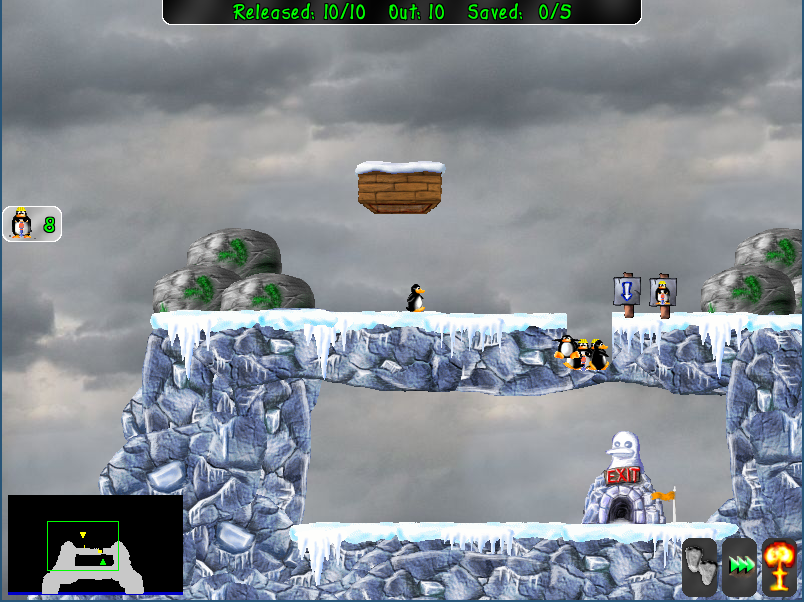
\includegraphics[width=\columnwidth]{pingus}
\caption{Pingus gameplay.
\label{fig.pingus}
}
\end{figure}

Pingus is an open-source puzzle-platform video game based on Lemmings.
The objective of the game is to guide a group of penguins through a number of
obstacles towards a designated exit (Figure~\ref{fig.pingus}).
% \footnote{Pingus gameplay video: \url{www.youtube.com/watch?v=MKrJgIFtJX0}}.
%
Pingus is developed in standard object-oriented C++, the \emph{lingua franca}
of game development \cite{games.patterns}.
The codebase%
\footnote{Pingus repository: \url{github.com/Pingus/pingus/}}
is about 40.000 lines of code (LoCs), divided into
the engine, level editor, auxiliary libraries, and the game logic itself.

According to Tim Sweeney (of Unreal Engine fame), about half the complexity in
game development resides in \emph{simulation} (aka \emph{game logic}), but
which accounts for only 10\% of the CPU budget~\cite{games.sweeney}
(Figure~\ref{fig.sweeney}).
%The game logic ``models the state of the game world as interacting objects
%evolve over time''.
The high development costs contrasting with the low impact on performance
appeals for alternatives with productivity in mind, especially considering that
it is the game logic that varies the most between projects.
Sweeney states that ``will gladly sacrifice 10\% of our performance for 10\%
higher productivity''.

\begin{figure}[t]
\centering
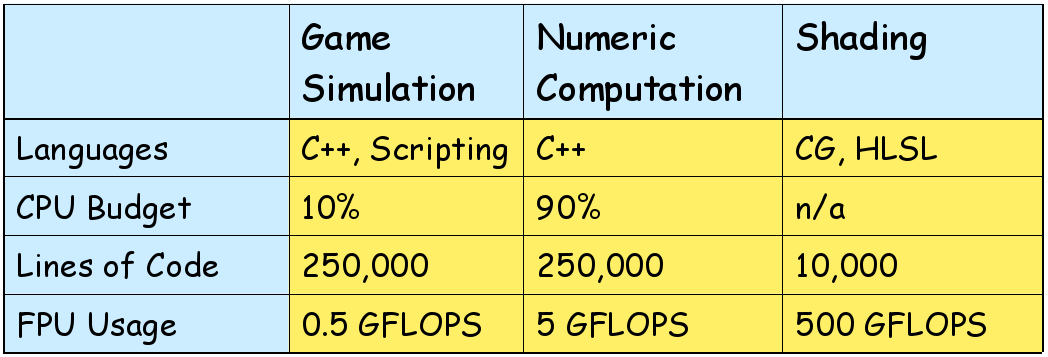
\includegraphics[width=\columnwidth]{sweeney}
\caption{Three kinds of code~\cite{games.sweeney}.
\label{fig.sweeney}
}
\end{figure}

Object-oriented games rely on the \emph{observer pattern}~\cite{games.patterns}
to handle events from the environment (e.g., key presses and timers) and also
as a notification mechanism between entities in the game logic.
%
The observers are short-lived callbacks that have to execute as fast as
possible to keep the game reactive to incoming events in real time.
%
For this reason, callbacks cannot contain long-lasting locals and loops, which
are elementary capabilities of classical structured
programming~\cite{rp.deprecating,rp.rescala,sync_async.cooperative}.
%
In this sense, callbacks actually disrupt structured programming, becoming
``our generation's \code{goto}''.%
\footnote{``Callbacks as our Generations' Go To Statement'':
\url{tirania.org/blog/archive/2013/Aug-15.html}}
%\footnote{``Escape from Callback Hell'':
%\url{elm-lang.org/learn/Escape-from-Callback-Hell.elm}}

\CEU~\cite{ceu.sensys13,ceu.mod15} is a programming language that offers a
concurrent and expressive alternative to C/C++ with the characteristics that
follow:
%
\begin{itemize}
\item \emph{Reactive}: code only executes in reactions to events.
\item \emph{Structured}: programs use structured control mechanisms, such as
      \code{await} (to suspend a line of execution), and \code{par} (to combine
      multiple lines of execution).
\item \emph{Synchronous}: reactions run atomically and to completion on each
      line of execution, i.e., there's no implicit preemption or real
      parallelism.
\end{itemize}
%
Structured reactive programming eliminates callbacks, letting programmers write
code in direct and sequential style and recover from the inversion of control
imposed by the observer pattern~\cite{rp.deprecating}.
%
\CEU supports logical parallelism with a resource-efficient implementation in
terms of memory and CPU usage~\cite{ceu.sensys13}.
The runtime is single threaded and does not rely on garbage collection.

In this work, we advocate structured synchronous reactive programming as an
expressive and productive alternative for game logic development.
We present a case study of rewriting Pingus from C++ to \CEU with the
contributions as follows:
%
\begin{itemize}
\item Identifying five recurrent control-flow patterns that likely apply to
      other games:
        \emph{Finite State Machines},
        \emph{Continuation Passing},
        \emph{Dispatching Hierarchies},
        \emph{Lifespan Hierarchies},
        \emph{Signaling Mechanisms}.
\item Applying idiomatic code in \CEU as alternative solutions for six selected
      behaviors in the game logic.
\item Presenting an in-depth qualitative analysis of the proposed solutions in
      comparison to the original implementations in C++.
\end{itemize}
%
A control-flow pattern is a recurring technique to describe dependencies and
explicit orders between statements (or groups of statements) in a program.
For instance, consider how a key press stimulus propagates through the game
entities and also what happens with them if the stimulus causes the end of the
game.
%
\CEU supports primitives that help describing complex control-flow
relationships in the game logic more concisely.
%
The rewriting process consisted of identifying sets of callbacks implementing
control flow in the game and translating them to \CEU using appropriate
structured constructs.
%
As an example, a double mouse click is characterized by a first click, followed
by a maximum amount of time, followed by a second click.
This behavior depends on different events (clicks and timers) which have to
occur in a particular order.
In C++, the implementation involves callbacks crossing reactions to successive
events which manipulate state variables explicitly.
%
Although we documented in detail two use cases for each of the five patterns,
in this work we only present six cases due to space constraints.
%
This work focuses on a qualitative analysis for the programming techniques
that we applied during the rewriting process.
Not all techniques result in reduction in LoCs (especially considering the
verbose syntax of \CEU), but have other effects such as eliminating shared
variables and dependencies between classes.

The rest of the paper is organized as follows:
Section~\ref{sec.codebase} gives an overview of the Pingus codebases in C++ and
\CEU.
Section~\ref{sec.patterns} describes the five control-flow patterns and
discusses six case studies in detail.
Section~\ref{sec.related} discusses related work.
Section~\ref{sec.conclusion} concludes the paper.

\section{The Pingus Codebase}
\label{sec.codebase}

\begin{figure*}[t]
\begin{verbatim}
Path              Ceu      C++   Ceu/C++    Descritpion
------------     ----     ----     ----     --------------------------------------------
game/            2064     2268     0.91     the main gameplay
  ./              710      679     1.05         main functionality
  objs/           470      478     0.98         world objects (tiles, traps, etc)
  pingu/          884     1111     0.80         pingu behaviors
    ./            343      458     0.75             main functionality
    actions/      541      653     0.83             pingu actions (bomber, climber, etc)
worldmap/         468      493     0.95     campaign worldmap
screens/         1109     1328     0.84     menus and screens
    option/       347      357     0.97         option menu
    others/       762      971     0.78         other menus and screens
misc/              56       46     1.22     miscellaneous functionality
                 ----     ----     ----
                 3697     4135     0.89
\end{verbatim}
\caption{The Pingus codebase directory tree.
\label{tab.tree}
}
\end{figure*}

In Pingus, the game logic also accounts for almost half the size of the
codebase: 18.173 from 39.362 LoCs (46\%) spread across 272 files.
%
However, about half of the game logic relates to non-reactive code, such as
configurations and options, saved games and serialization, maps and levels
descriptions, string formatting, collision detection, graph algorithms, etc.
This part remains unchanged and relies on the seamless integration between \CEU
and C/C++~\cite{ceu.sensys13}.
%
Therefore, we rewrote 9.186 LoCs spread across 126 files%
\footnote{Complete codebase: \url{github.com/an000/p/tree/master/cpp}}.
%
In order to only consider effective code in the analysis, we then removed all
headers, declarations, trivial getters \& setters, and other innocuous
statements, resulting 4.135 dense LoCs spread across 70 implementation files
originally written in C++%
\footnote{C++ codebase: \url{github.com/an000/p/tree/master/all}}.
We did the same with the implementation in \CEU, resulting in 3.697 dense LoCs%
\footnote{\CEU codebase: \url{github.com/an000/p/tree/master/all}}.
%
Figure~\ref{tab.tree} summarizes the effective codebase in the two
implementations.

%%%
This work focuses on a qualitative analysis for the programming techniques
that we applied during the rewriting process.
Not all techniques result in reduction in LoCs (especially considering the
verbose syntax of \CEU), but have other effects such as eliminating shared
variables and dependencies between classes.
%<!--, helping on encapsulation and cohesion.-->
Nonetheless, the lines with lower ratio numbers above correlate to the parts of
the game logic that we consider more susceptible to structured reactive
programming.
For instance, the \emph{Pingu} behavior (\emph{ratio 0.80}) contains complex
animations that are affected by timers, game rules, and user interaction.
In contrast, the \emph{Option screen} (\emph{ratio 0.97}) is a simple UI grid
with trivial mouse interactions.
%%%

\section{Control-Flow Patterns \& Case Studies}
\label{sec.patterns}

TODO: state pattern, FSM
      strategy/visitor pattern, polymorhpism, hierarchies
      observer pattern, signaling


use cases first -> patterns later

We can identify control-flow behaviors in C++ by looking for class members with
identifiers resembling verbs, statuses, and counters (e.g.,
\code{pressed},
\code{particle\_thrown},
\code{mode}, and
\code{delay\_count}).
Good chances are that variables with these ``suspicious names'' encode some
form of control-flow progression that cross multiple callback invocations.

We selected 6 representative game behaviors and describe their
implementations in C++ and \CEU.
We also categorize these behaviors in 5 abstract control-flow patterns that
likely apply to other games:

\begin{enumerate}
\item \emph{Finite State Machines}:
    Event occurrences map to transitions between states that trigger
    appropriate actions comprising the behavior of a game entity.
\item \emph{Continuation Passing}:
    The completion of a long-lasting activity may carry a continuation, i.e.,
    some action to execute next in the game.
\item \emph{Dispatching Hierarchies}:
    Entities form a dispatching hierarchy in which a container that receives a
    stimulus automatically forwards it to its managed children.
\item \emph{Lifespan Hierarchies}:
    Entities form a lifespan hierarchy in which a terminating container entity
    automatically destroys its managed children.
\item \emph{Signaling Mechanisms}:
    Entities often need to communicate and affect each other explicitly through
    signaling mechanisms, especially if there is no hierarchy relationship
    between them.
\end{enumerate}

\subsection{Finite State Machines}

TODO: falar do state pattern, citar game.patterns, falar que usa estado explicito

\textbf{Case Study: Detecting double-clicks in the \emph{Armageddon button}}

%\begin{figure}[t]
%\centering
%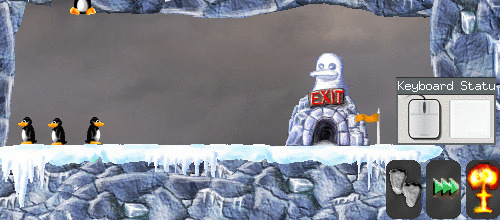
\includegraphics[width=\columnwidth]{double-click-opt}
%\caption{Double click detection.
%\label{fig.armageddon}
%}
%\end{figure}
%(Figure~\ref{fig.armageddon}).

In Pingus, a double click in the \emph{Armageddon button} at the bottom right
of the screen literally explodes all pingus.%
\footnote{Double click animation: \url{github.com/an000/p/blob/master/README.md#1} }

\begin{figure*}[t]
\begin{minipage}[t]{0.55\linewidth}
\begin{lstlisting}[numbers=left,xleftmargin=3em]
ArmageddonButton::ArmageddonButton(<...>):
    RectComponent(<...>),
    pressed(false); // button initially not pressed
    press_time(0);    // how long since 1st click?
    <...>
{
    <...>
}

void ArmageddonButton::draw (<...>) {
    <...>
}

void ArmageddonButton::update (float delta) {
    <...>
    if (pressed) {
        press_time += delta;
        if (press_time > 1.0f) {
            pressed = false; // give up, 1st click
            press_time = 0;  // was too long ago
        }
    } else {
        <...>
        press_time = 0;
    }
}

void ArmageddonButton::on_click (<...>) {
    if (pressed) {
        send_armageddon_event();
    } else {
        pressed = true;
    }
}
\end{lstlisting}
\centering\small{\ax Implementation in C++}
\end{minipage}
%
\begin{minipage}[t]{0.45\linewidth}
\begin{lstlisting}[numbers=left,xleftmargin=3em]
do
    var RectComponent c = <...>;
    <...>
    loop do
        await c.component.on_click;
        watching 1s do
            await c.component.on_click;
            break;
        end
    end
    <...>
    emit game.go_armageddon;
end




















.
\end{lstlisting}
\centering\small{\bx Implementation in \CEU}
\end{minipage}
%\rule{8.4cm}{0.37pt}
\caption{ Detecting double-clicks in the \emph{Armageddon button}.
\label{lst.armageddon}
}
\end{figure*}

Figure~\ref{lst.armageddon}.a shows the C++ implementation for the class
\code{ArmageddonButton} with methods for rendering the button and handling
mouse and timer events.
The code focus on the double click detection and hides unrelated parts with
\code{<...>}.
%
The methods \code{update} (ln. 14--26) and \code{on\_click} (ln. 28--34) are
examples of \emph{short-lived callbacks}, which are pieces of code that execute
atomically in reaction to external input events.
The callback \code{on\_click} reacts to mouse clicks detected by the base class
\code{RectComponent} (ln. 2), while the callback \code{update} continuously
reacts to the passage of time, frame by frame.
Callbacks are short lived because they must react to input as fast as possible
to let other callbacks execute, keeping the game with real-time responsiveness.
%
The class first initializes the variable \code{pressed} to track the first
click (ln. 3,32).
It also initializes the variable \code{press\_time} to count the time since the
first click (ln. 4, 17).
If another click occurs within 1 second, the class signals the double click to
the application (ln. 30).
Otherwise, the \code{pressed} and \code{press\_time} state variables are reset
(ln. 19--20). 
%
Figure~\ref{fig.armageddon.fsm} illustrates how we can model the double-click 
behavior in C++ as a state machine.
The circles represent the state of the variables in the class, while the arrows 
represent the callbacks manipulating state.
%
Note in the code how the accesses to the state variables are spread
across the entire class.
For instance, the distance between the initialization of \code{pressed} (ln.
3) and the last access to it (ln. 32) is over 40 lines in the original file.
Arguably, this dispersion of code across methods makes the understanding and 
maintenance of the double-click behavior more difficult.
Also, even though the state variables are private, unrelated methods such as 
\code{draw}, which is defined in middle of the class (ln. 10--12), can
potentially access them.

\begin{figure}[t]
\centering
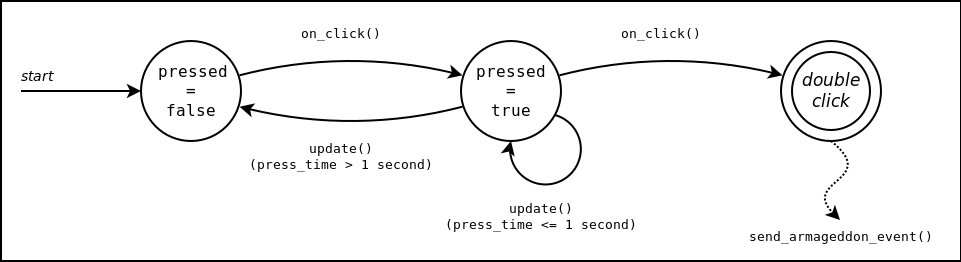
\includegraphics[width=\columnwidth]{double-click}
\caption{State machine for detecting double-clicks in the
         \emph{Armageddon button}.
\label{fig.armageddon.fsm}
}
\end{figure}

\CEU provides structured constructs to deal with events, aiming to eradicate
explicit manipulation of state variables for control-flow purposes.
%
In Figure~\ref{lst.armageddon}.b, the loop detection (ln. 4--10) awaits the
first click (ln. 5) and then, while watching 1 second (ln. 6--9), awaits the
second click (ln. 7).
If the second click occurs within 1 second, the \code{break} terminates the
loop (ln. 8) and the \code{emit} signals the double click to the application
(ln. 12).
Otherwise, the \code{watching} block as a whole aborts after 1 second  and the
loop restarts, falling back to the first click \code{await} (ln. 5).
%
Double click detection in \CEU doesn't require state variables and is entirely
self-contained in the \code{loop} body (ln. 4--10).
Also, these 7 lines of code \emph{only} detect the double click, leaving the
actual effect to happen outside the loop (ln. 12).

TODO: Structured programming, ...

\textbf{Case Study: The \emph{Bomber action} animation sequence}

TODO: descrever o que sao actions, exibir imagem da tela com menu de actions e
seta apontando para pingu sendo clicado e com acao recem ativada

%\begin{figure}[t]
%\centering
%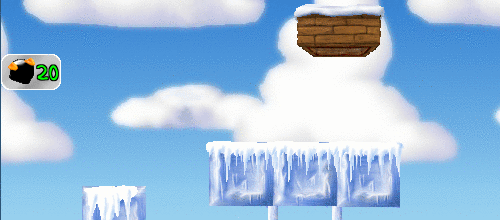
\includegraphics[width=\columnwidth]{bomber-anim}
%\caption{ The \emph{Bomber action}.
%\label{fig.bomber.anim}
%}
%\end{figure}

\begin{figure}[t]
\centering
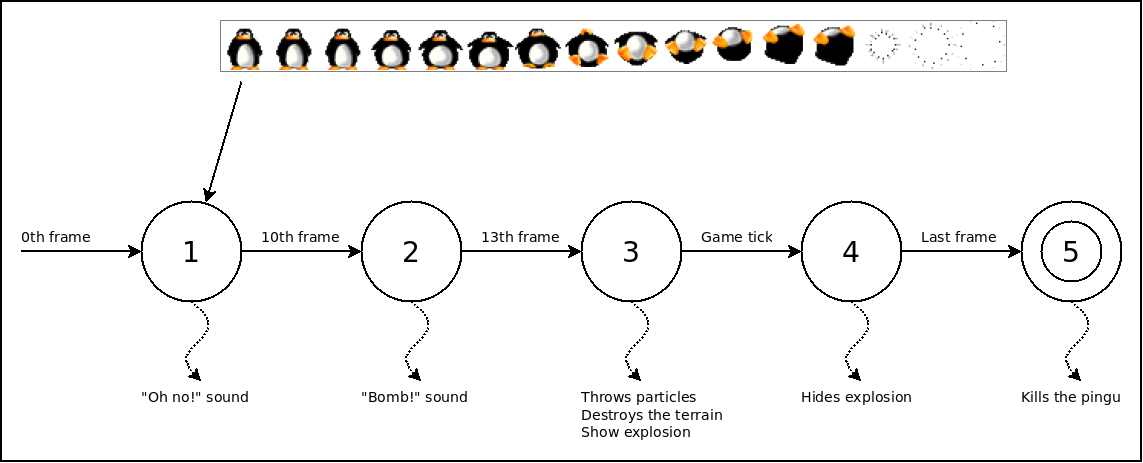
\includegraphics[width=\columnwidth]{bomber-state}
\caption{ State machine for the \emph{Bomber animation} sequence.
\label{fig.bomber}
}
\end{figure}

\begin{figure*}[th!]
\begin{minipage}[t]{0.50\linewidth}
\begin{lstlisting}[numbers=left,xleftmargin=3em]
Bomber::Bomber (Pingu* p) :
  <...>
  sprite(<...>),          // bomber sprite
  sound_played(false),    // tracks state 2
  particle_thrown(false), // tracks state 3
  colmap_exploded(false), // tracks state 3
  gfx_exploded(false)     // tracks state 4
{
  <...>
  // 1. plays a "Oh no!" sound.
  play_sound("ohno");
}

void Bomber::update () {
  sprite.update();
  <...>   // pingu movement

  // 2. plays a "Bomb!" sound.
  if (sprite.frame()==10 && !sound_played) {
    sound_played = true;
    play_sound("plop");
  }

  // 3. particles, terrain, explosion sprite
  if (sprite.frame()==13 && !particle_thrown) {
    particle_thrown = true;
    get_world()->get_particles()->add(...);
  }
  if (sprite.frame()==13 && !colmap_exploded) {
    colmap_exploded = true;
    get_world()->remove(bomber_radius, <...>);
  }

  // 5. kills the Pingu
  if (sprite.is_finished ()) {
    pingu->set_status(PS_DEAD);
  }
}

void Bomber::draw (SceneContext& gc) {
  // 3. particles, terrain, explosion sprite
  // 4. tick: hides the explosion sprite
  if (sprite.frame()==13 && !gfx_exploded) {
    gfx_exploded = true;
    gc.color().draw(explo_surf, <...>);
  }
  gc.color().draw(sprite, pingu->get_pos());
}
\end{lstlisting}
\centering\small{\ax Implementation in C++}
\end{minipage}
%
\begin{minipage}[t]{0.50\linewidth}
\begin{lstlisting}[numbers=left,xleftmargin=3em]
code/await Bomber (void) -> ActionName
do
  <...>
  spawn Mover();  // movement in the background
  var Sprite s = spawn Sprite(<...>);
                  // animation in the background
  watching s do
    // 1. plays a "Oh no!" sound.
    {play_sound("ohno")};

    // 2. plays a "Bomb!" sound.
    await game.dt until s.sprite.frame == 10;
    {play_sound("plop")};

    // 3. particles, terrain, explosion sprite
    await game.dt until s.sprite.frame == 13;
    spawn PinguParticles(<...>) in particles;
    call Game_Remove({&bomber_radius}, <...>);
    do
      <...>
      spawn Sprite(<...>);      // explosion

      // 4. tick: hides the explosion sprite
      await game.dt;
    end
    await FOREVER;
  end

  // 5. kills the pingu
  escape DEAD;
end
















.
\end{lstlisting}
\centering\small{\bx Implementation in \CEU}
\end{minipage}
%\rule{8.4cm}{0.37pt}
\caption{ The \emph{Bomber action} sequence.
\label{lst.bomber}
}
\end{figure*}

The \emph{Bomber action} explodes the clicked pingu, throwing particles around
and also destroying the terrain under its radius.%
\footnote{Bomber action animation: \url{github.com/an000/p/blob/master/README.md#2} }
%
We can model the explosion animation with a sequential state machine
(Figure~\ref{fig.bomber}) with actions associated to specific frames as
follows%
\footnote{State machine animation: \url{github.com/an000/p/blob/master/README.md#3} }:
%
\begin{enumerate}
\item 0th frame:  plays a "Oh no!" sound.
\item 10th frame: plays a "Bomb!" sound.
\item 13th frame: throws particles, destroys the terrain, and shows an
                  explosion sprite.
\item Game tick:  hides the explosion sprite.
\item Last frame: kills the pingu.
\end{enumerate}

Figure~\ref{lst.bomber} compares the implementations in C++ and \CEU.

In C++, the class \code{Bomber} defines the callbacks \code{draw} and
\code{update} to manage the state machine described above.
%
The class first defines one state variable for each action to perform
(ln. 4--7).
The ``Oh no!'' sound plays as soon as the object starts in \emph{state-1} 
(ln. 11).
The \code{update} callback (ln. 14--38) first updates the pingu animation and
movement on every frame regardless of its current state (ln. 15--16).
When the animation reaches the 10th frame, it plays the ``Bomb!'' sound and 
switches to \emph{state-2} (ln. 18--22).
The state variable \code{sound\_played} is required because the sprite frame
doesn't necessarily advance on every \code{update} invocation (e.g.,
\code{update} may execute twice during the 10th frame).
The same reasoning and technique applies to \emph{state-3} (ln. 24--32 and
43--44).
The explosion sprite appears in a single frame in \emph{state-4} (ln. 45).
Finally, the pingu dies after the animation frames terminate (ln. 34--35).
%
Note that a single numeric state variable suffices to track the states, but the
original authors probably chose to encode each state in an independent boolean 
variable to rearrange and experiment with them during development.
Still, due to the short-lived nature of callbacks, state variables are 
unavoidable and are actually the essence of object-oriented programming
(i.e., \emph{methods + mutable state}).
%
Like double click detection in C++, note that the state machine is encoded
across 3 different methods, each intermixing code with unrelated functionality.

The equivalent code for the \emph{Bomber action} in \CEU doesn't require state
variables and reflects the sequential state machine implicitly, using
\code{await} statements in direct style to separate the actions.
%
The \code{Bomber} is a \code{code/await} abstraction of \CEU, which is similar
to a coroutine or fiber~\cite{sync_async.cooperative}: a subroutine that
retains runtime state, such as local variables and the program counter, across
reactions to events (i.e., across \code{await} statements).
The pingu movement and sprite animation are isolated in two other
\code{code/await} abstractions and execute in separate through the \code{spawn}
primitive (ln. 4--5).
The event \code{game.dt} (ln. 12,16,24) is analogous to the \code{update}
callback of C++ and occurs on every frame.
%
The code tracks the animation aliveness (ln. 7--27) and, on termination,
performs the last bomber action (ln. 30).
As soon as the animation starts, the code performs the first action (ln. 9).
The intermediate actions are performed when the corresponding conditions occur
(ln. 12,16,24).
The \code{do-end} block (ln. 19--25), restricts the lifespan of the
single-frame explosion sprite (ln. 21): after the next game tick (ln. 24), the
block terminates and automatically destroys the spawned abstraction (removing
it from the screen).
%
In contrast with the implementation in C++, all actions happen in a contiguous
chunk of code (ln. 5--30) which handles no extra functionality.

\subsection{Continuation Passing}

TODO: what is this?

\textbf{Case Study: Advancing Pages in the \emph{Story screen}}

%\begin{figure}[t]
%\centering
%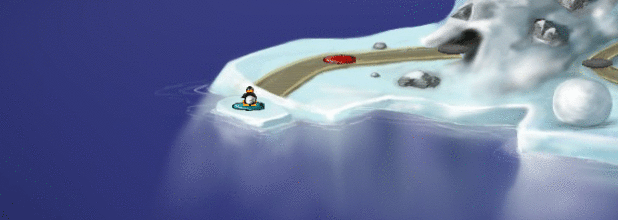
\includegraphics[width=\columnwidth]{story-anim}
%\caption{The \emph{Story screen}.
%\label{fig.story}
%}
%\end{figure}

\begin{figure}[t]
\centering
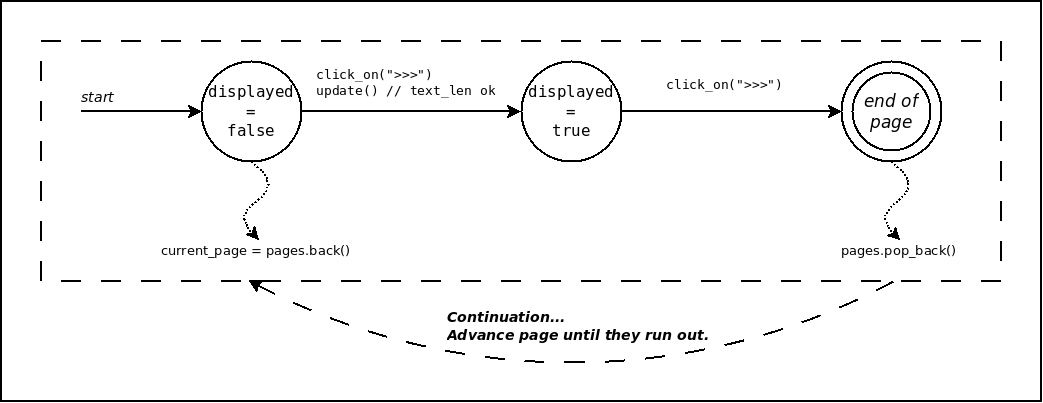
\includegraphics[width=\columnwidth]{story}
\caption{State machine for advancing pages in the \emph{Story screen}.
\label{fig.story}
}
\end{figure}

\begin{figure*}[t]
\begin{minipage}[t]{0.55\linewidth}
\begin{lstlisting}[numbers=left,xleftmargin=3em]
StoryScreenComponent::StoryScreenComponent (<...>) :
    <...>
{
    pages        = <...>; // vector with loaded pages
    current_page = pages.back(); // first loaded page
    displayed    = false; // if current is complete
    <...>
}

<...>   // draw page over time

void StoryScreenComponent::update (<...>) {
    <...>
    if (<all-words-appearing>) {
        displayed = true;
    }
}

void StoryScreenComponent::next_text() {
    if (!displayed) {
        displayed = true;
        <...>     // remove current page
    } else {
        pages.pop_back();
        if (!pages.empty()) { // next page
            current_page = pages.back();
            displayed    = false;
            <...>
        } else {
            <...> // terminates the story screen
        }
    }
}
\end{lstlisting}
\centering\small{\ax Implementation in C++}
\end{minipage}
%
\begin{minipage}[t]{0.45\linewidth}
\begin{lstlisting}[numbers=left,xleftmargin=3em]
code/await Story (void) -> bool do
    <...>
    event void next_text; // clicks in >>>

    { pages = <...>; } // same as in C++
    loop i in [0 <- {pages.size()}[ do
        par/or do
            watching next_text do
                <...> // advance text
            end
            await next_text;
        with
            <...> // redraw _pages[i]
        end
    end
end

















.
\end{lstlisting}
\centering\small{\bx Implementation in \CEU}
\end{minipage}
%\rule{8.4cm}{0.37pt}
\caption{ Advancing pages in the \emph{Story Screen}.
\label{lst.story}
}
\end{figure*}

The clickable \emph{blue dots} in the campaign world map transit to ambience
story screens%
\footnote{Story screen animation: \url{github.com/an000/p/blob/master/README.md#4} }.
A story is composed of multiple pages and, inside each page, the words of the
story appear incrementally over time.
A first click in the button \code{>>>} fast forwards the words to show the full 
page.
A second click advances to the next page, until the story terminates.
If the page completes before a click (due to the time elapsing), a first click 
advances to the next page.
%
Figure~\ref{lst.story} compares the implementations in C++ and \CEU.

In C++, the class \code{StoryScreenComponent} implements the method
\code{next\_text}, which is a callback for clicks in \code{>>>}.
%
The variable `pages` (ln. 4--5, 24--26) is a vector holding each page, but
which also encodes \emph{continuations} for the story progress:
each call to \code{next\_text} that advances the story (ln. 23--32) removes the 
current page (ln. 24) and sets the next action to perform (i.e., ``display a
new page'') in the variable \code{current\_page} (ln. 26).
Figure~\ref{fig.story} illustrates the continuation mechanism to advance 
pages and also a state machine for fast forwarding words (inside the dashed
rectangle).
The state variable \code{displayed} (ln. 6,15,20,21,27) switches between the
behaviors ``advancing text'' and ``advancing pages'', which are both handled
intermixed inside the method \code{next\_text}.

The code in \CEU uses the internal event \code{next\_text}, which is emitted
from clicks in \code{>>>}.
%
The sequential navigation from page to page uses a loop in direct style
(ln. 6--15) instead of explicit state variables for the continuation and state
machine.
While the text advances in an inner loop (hidden in ln. 9), we watch the
\code{next\_text} event that fast forwards it.
The loop may also eventually terminate with the time elapsing normally.
This way, we do not need a variable (such as `displayed` in C++) to switch 
between the states ``advancing text'' and ``advancing pages''.
The \code{par/or} makes the page advance logic to execute in parallel with the
redrawing code (ln. 13).
Whenever the page advances, the redrawing code is automatically aborted
(due to the \code{or} modifier).
The \code{await next\_text} in sequence (ln. 11) is the condition to advance to
the next page.
%
Note that, unlike the implementation in C++, the ``advancing text'' behavior is
not intermixed with the ``advancing pages'' behavior, instead, it is
encapsulated inside the inner loop nested with a deeper indentation (ln. 9).

\subsection{Dispatching Hierarchies}

\textbf{Case Study: \emph{Bomber action} \code{draw} and \code{update} dispatching}

TODO

Figure~\ref{lst.hier} compares the implementations in C++ and \CEU.

\begin{figure}[t]
\centering
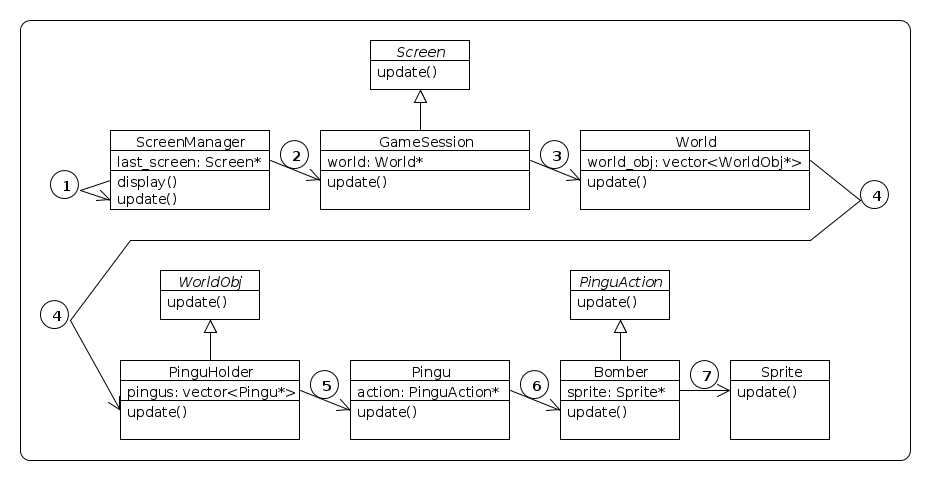
\includegraphics[width=\columnwidth]{hierarchy}
\caption{Dispatching chain for \code{update}.
\label{fig.hier}
}
\end{figure}

\begin{figure*}[t]
\begin{minipage}[t]{0.50\linewidth}
\begin{lstlisting}[numbers=left,xleftmargin=3em]
class Bomber : public PinguAction {
    <...>
    Sprite sprite;
}

Bomber::Bomber (<...>) : <...> {
    sprite.load(<...>);
    <...>
}

void Bomber::update () {
    sprite.update ();
}

void Bomber::draw (SceneContext& gc) {
    <...>
    gc.color().draw(sprite, <...>);
}
\end{lstlisting}
\centering\small{\ax Implementation in C++}
\end{minipage}
%
\begin{minipage}[t]{0.50\linewidth}
\begin{lstlisting}[numbers=left,xleftmargin=3em]
code/await Bomber (void) -> ActionName do
    <...>
    var&? Sprite sprite = spawn Sprite(<...>);
    <...>
end












.
\end{lstlisting}
\centering\small{\bx Implementation in \CEU}
\end{minipage}
%\rule{8.4cm}{0.37pt}
\caption{ \emph{Bomber action} \code{draw} and \code{update} dispatching.
\label{lst.hier}
}
\end{figure*}

In C++, the class \code{Bomber} declares a \code{sprite} member to handle its
animation frames (Figure~\ref{fig.bomber}).
%
The \code{Sprite} class is part of the game engine and knows how to update and
render itself.
However, the \code{Bomber} still has to respond to \code{update} and
\code{draw} requests from the game and forward them to the sprite
(ln. 11--13 and 15--18).
%
To understand how the \code{update} callback flows from the original
environment stimulus from the game down to the sprite, we need to follow a long
chain of 7 method dispatches (Figure~\ref{fig.hier}):
%
\begin{enumerate}
\item \code{ScreenManager::display} in the main game loop calls \code{update}.
\item \code{ScreenManager::update} calls \code{last\_screen->update} for the
      active game screen (a \code{GameSession} instance, considering the
      \code{Bomber}).
\item \code{GameSession::update} calls \code{world->update}.
\item \code{World::update} calls \code{obj->update} for each object in the
      world.
\item \code{PinguHolder::update} calls \code{pingu->update} for each pingu
      alive.
\item \code{Pingu::update} calls \code{action->update} for the active pingu
      action.
\item \code{Bomber::update} calls \code{sprite.update}.
      \code{Sprite::update} finally updates the animation frame.
\end{enumerate}
%
Each dispatching step in the chain is necessary considering the game
architecture:
%
\begin{itemize}
\item With a single assignment to \code{last\_screen}, we can easily deactivate
      the current screen and redirect all dispatches to a new screen.
\item The \code{World} class manages and dispatches events to all game
      entities, such as all pingus and traps, with the common interface
      \code{WorldObj}.
\item Since it is common to iterate only over the pingus (vs. all world
      objects), the container \code{PinguHolder} manages all pingus.
\item Since a single pingu can change between actions during lifetime, the
      \code{action} member decouples them with another level of indirection.
\item Sprites are part of the game engine and are reusable everywhere (e.g., UI
      buttons, world objects, etc.), so it is also convenient to decouple them
      from actions.
\end{itemize}
%
The \code{draw} callback flows through the same dispatching hierarchy until
reaching the \code{Sprite} class.

In \CEU, the \code{Bomber} action spawns a \code{Sprite} animation instance on
its body.
%
The \code{Sprite} instance (ln. 3) can react directly to external \code{dt} and
\code{redraw} events (which are analogous to \code{update} and \code{redraw}
callbacks, respectively), bypassing the program hierarchy entirely.
While and \emph{only while} the bomber abstraction is alive, the sprite
animation is also alive.
The radical decoupling between the program hierarchy and reactions to events
eliminates dispatching chains entirely.

\subsection{Lifespan Hierarchies}

\textbf{Case Study: Managing the Pingus Lifecycle}

%\begin{figure}[t]
%\centering
%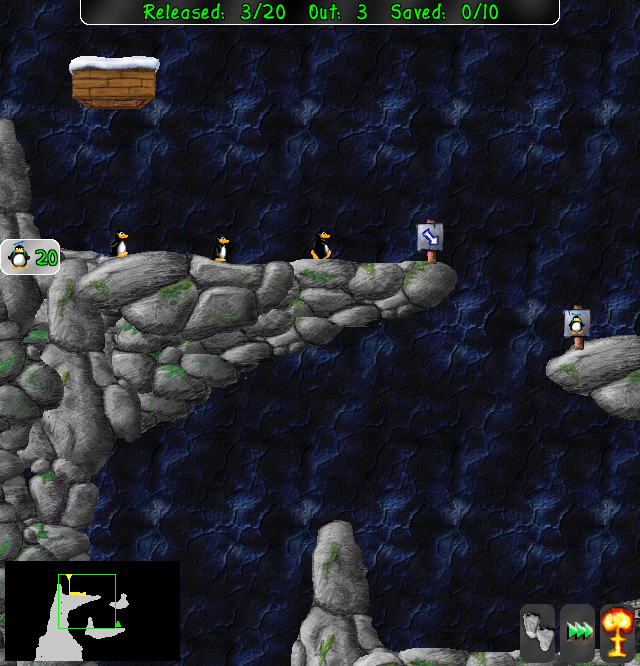
\includegraphics[width=\columnwidth]{pingus_create_die-anim}
%\caption{Creation and death of pingus.
%\label{fig.pingus_create_die}
%}
%\end{figure}

A pingu is a dynamic entity created periodically and destroyed under certain
conditions, such as falling from a high altitude%
\footnote{Death of pingus animation: \url{github.com/an000/p/blob/master/README.md#5} }.
%
Figure~\ref{lst.pingus} compares the implementations in C++ and \CEU.

\begin{figure*}[t]
\begin{minipage}[t]{0.50\linewidth}
\begin{lstlisting}[numbers=left,xleftmargin=3em]
Pingu* PinguHolder::create_pingu (<...>) {
    <...>
    Pingu* pingu = new Pingu (<...>);
    pingus.push_back(pingu);
    <...>
}

void PinguHolder::update() {
    <...>
    while(pingu != pingus.end()) {
        (*pingu)->update();
        if ((*pingu)->get_status() == PS_DEAD) {
            pingu = pingus.erase(pingu);
        }
        <...>
        ++pingu;
    }
}

.
\end{lstlisting}
\centering\small{\ax Implementation in C++}
\end{minipage}
%
\begin{minipage}[t]{0.50\linewidth}
\begin{lstlisting}[numbers=left,xleftmargin=3em]
code/await Game (void) do
    <...>
    pool[] Pingu pingus;
    code/await Pingu_Spawn (<...>) do
        <...>
        spawn Pingu(<...>) in pingus;
    end
    <...>   // code invoking Pingu_Spawn
end

code/await Pingu (<...>) do
    <...>
    loop do
        await game.dt;
        if Pingu_Is_Out_Of_Screen() then
            <...>
            escape {PS_DEAD};
        end
    end
end
\end{lstlisting}
\centering\small{\bx Implementation in \CEU}
\end{minipage}
%\rule{8.4cm}{0.37pt}
\caption{ Managing the pingus lifecycle.
\label{lst.pingus}
}
\end{figure*}

In C++, the class \code{PinguHolder} is a container that holds all pingus
alive.
%
The method \code{PinguHolder::create\_pingu} (ln. 1--6) is called periodically
to create a new \code{Pingu} and add it to the \code{pingus} collection
(ln. 3--4).
The method \code{PinguHolder::update} (ln. 8--18) checks the state of all
pingus on every frame, removing those with the dead status (ln. 12--14).
%
Entities with dynamic lifespan in C++ require explicit \code{add} and
\code{remove} calls associated to a container (ln. 4,13).
Without the \code{erase} call above, a dead pingu would remain in the
collection with updates on every frame (ln. 11).
Since the \code{redraw} behavior for a dead pingu is innocuous, the death could
go unnoticed but the program would keep consuming memory and CPU time.
This problem is known as the \emph{lapsed listener}~\cite{games.patters} and
also occurs in languages with garbage collection:
A container typically holds a strong reference to a child (sometimes the only 
reference to it), and the runtime cannot magically detect it as garbage.

\begin{figure}[t]
\centering
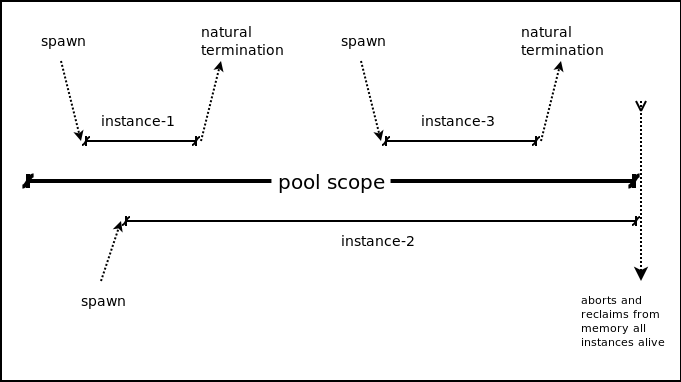
\includegraphics[width=\columnwidth]{pool}
\caption{Lifespan of dynamic instances.
\label{fig.pool}
}
\end{figure}

\CEU supports \code{pool} declarations to hold dynamic abstraction instances.
Additionally, the \code{spawn} statement supports a pool identifier to
associate the new instance with a pool.
%
The game screen spawns a new \code{Pingu} on every invocation of
\code{Pingu\_Spawn}.
%
The \code{spawn} statement (ln. 6) specifies the pool declared at the top-level
block of the game screen (ln. 3).
In this case, the lifespan of the new instances follows the scope of the pool
(ln. 1--9) instead of the enclosing scope of the \code{spawn} statement
(ln. 4--7).
Since pools are also subject to lexical scope, the lifespan of all dynamically
allocated pingus is constrained to the game screen.
%
Lexical scopes handle memory and event dispatching automatically for static
instances and also for pools.
However, the lifespan of a dynamic instance does not necessarily have to match
the lifespan of its associated pool (Figure~\ref{fig.pool}).
In \CEU, when the execution block of a dynamic instance terminates, which
characterizes its \emph{natural termination}, the instance is automatically
removed from its pool.
Therefore, dynamic instances do not require any extra bookkeeping related to 
containers or explicit deallocation.
%
To remove a pingu from the game in \CEU, we just need to terminate its execution
block according to the appropriate conditions:
%
The \code{escape} statement (ln. 17) aborts the execution block of the
\code{Pingu} instance, removing it from its associated pool automatically.
Hence, a dynamic instance that terminates naturally leaves no traces in the 
program.

\subsection{Signaling Mechanisms}

\textbf{Case Study: Global Keys and the Options Menu}

%\begin{figure}[t]
%\centering
%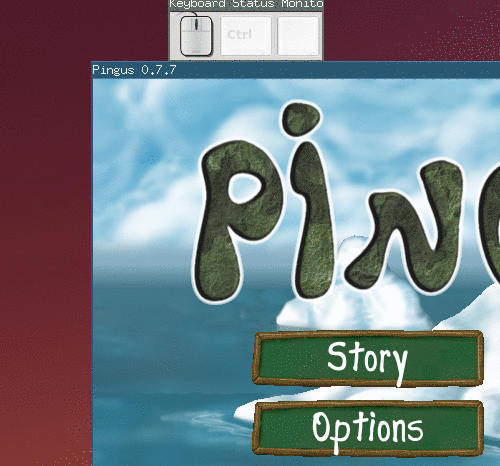
\includegraphics[width=\columnwidth]{options-anim-opt}
%\caption{The \emph{Mouse Grab} configuration option.
%\label{fig.options}
%}
%\end{figure}

\begin{figure}[t]
\centering
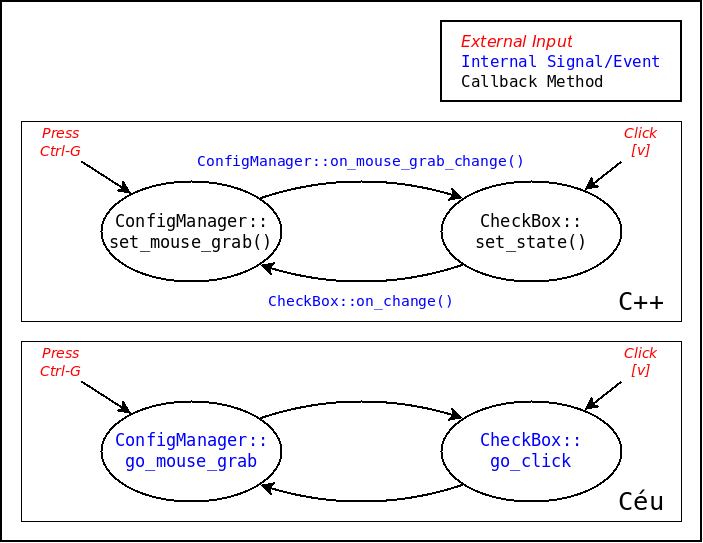
\includegraphics[width=\columnwidth]{events}
\caption{Mutual dependency between signals.
\label{fig.events}
}
\end{figure}

\begin{figure*}[t]
\begin{minipage}[t]{0.50\linewidth}
\begin{lstlisting}[numbers=left,xleftmargin=3em]
void GlbEvt::on_button_press (<...>) {
  <...>
  switch (event.keysym.sym) {
    case K_g:
      if (keys[K_LCTRL] || keys[K_RCTRL]) {
        cfgmgr.set_grab(
          !cfgmgr.get_grab());
      }
      break;
    <...>
  }
}

///

boost::signal<void(bool)> on_grab_change;

void CfgMgr::set_grab (bool v) {
  <...>
  if (v != get_grab()) {
    <...>   // the actual "grab" effect
    on_grab_change(v);
  }
}

///

boost::signal<void (bool)> on_change;

void ChkBox::set (bool on, bool sndsig) {
  <...>   // switches the check box state
  if (sndsig) {
    on_change(on);
  }
}

///

typedef std::vector<boost::connection> Conns;
Conns conns;

OptMenu::OptMenu() :
  conns(),
  grab_box(),
  <...>
{
  grab_box = new ChkBox(<...>);
  conns.push_back(
    cfgmgr.on_grab_change.connect( std::bind(
      &ChkBox::set, grab_box, <...>, false) );
    )
  );
  conns.push_back(
    grab_box->on_change.connect( std::bind(
      &CfgMgr::set_grab, &cfgmgr, <...>) );
    )
  );
  <...>

}

OptMenu::~OptMenu() {
  for (Conns::iterator i=conns.begin();
             i!=conns.end();
             ++i) {
    (*i).disconnect();
  }
}


.
\end{lstlisting}
\centering\small{\ax Implementation in C++}
\end{minipage}
%
\begin{minipage}[t]{0.50\linewidth}
\begin{lstlisting}[numbers=left,xleftmargin=3em]
spawn do
  var _SDL_KeyboardEvent&& e;
  every e in SDL_KEYDOWN do
    var _u8&& keys = _SDL_GetKeyState(null);
    <...>
    if e:keysym.sym == K_g then
      if keys[K_LCTRL] or keys[K_RCTRL] then
        emit cfgmgr.go_grab(
            not {cfgmgr.get_grab()});
      end
    end
    <...>
  end
end

///

data CfgMgr with
  event bool go_grab;
end
var CfgMgr cfgmgr = val CfgMgr(_);

spawn do
  var bool v;
  every v in cfgmgr.go_grab do
    <...>   // the actual "grab" effect
  end
end

///

data IChkBox with
  var   bool is_on;
  event bool go_click;
end

code/await ChkBox (<...>) -> (var IChkBox box) -> FOREVER do
  box = val IChkBox(<...>);
  <...>
  par do
    every c.component.on_click do
      emit box.go_click(not box.is_on);
    end
  with
    loop do
      <...>   // switches the check box state
      box.is_on = await box.go_click;
    end
  end
end

///

code/await OptMenu <...> do
  <...>
  var& ChkBox b2 = <...>;
  spawn do
    par do
      var bool v;
      every v in cfgmgr.go_grab do
        emit b2.box.go_click(v);
      end
    with
      var bool v;
      every v in b2.box.go_click do
        emit cfgmgr.go_grab(v);
      end
    end
  end
  <...>
end
\end{lstlisting}
\centering\small{\bx Implementation in \CEU}
\end{minipage}
%\rule{8.4cm}{0.37pt}
\caption{ TODO.
\label{lst.grab}
}
\end{figure*}

The \emph{mouse grab option} restricts the mouse movement to the game window
boundaries%
\footnote{Mouse grab animation: \url{github.com/an000/p/blob/master/README.md#6} }.
The option can be set anywhere in the game by pressing \emph{Ctrl-G}.
In addition, the \emph{Options menu} has a check box to toggle the
\emph{mouse grab option} with mouse clicks while still responding to
\emph{Ctrl-G} presses.
%
Figure~\ref{lst.grab} compares the implementations in C++ and \CEU.

The implementations in C++ and \CEU use a signalling mechanism to connect the
key presses, the check box, and a configuration manager that applies the
appropriate side effects in the game (i.e., restrict the mouse movement).
Figure~\ref{fig.events} illustrates how the mutual notifications create a 
dependency cycle between the configuration manager and the check box.

In C++, the class `GlbEvt` detects \emph{Ctrl-G} presses and invokes the
callback \code{config\_manager.set\_grab} (ln. 5--8).
%
The class `CfgMgr` uses a \code{boost::signal} (ln. 16) to notify the
application when the new configuration is applied (ln. 22).
%
The \code{if} enclosing the signal emission (ln. 20--23) breaks the dependency 
cycle of Figure~\ref{fig.events} and prevents an infinite execution loop.
%
The class \code{ChkBox} also uses a \code{boost::signal} (ln. 28) to notify
the application on changes (ln. 33).
%
Again, the \code{if} enclosing the signal emission (ln. 32--34) breaks the 
dependency cycle of Figure~\ref{fig.events} to avoid infinite execution.
%
The class \code{OptMenu} creates the dependency loop by connecting the two
signals.
%
The constructor binds
the signal \code{config\_manager.on\_grab\_change} to the callback
    method \code{grab\_box->set} (ln. 48--52),
and also
the signal \code{grab\_box->on\_change} to the callback method
    \code{config\_manager.set\_grab} (ln. 53--57).
This way, every time the \code{CfgMgr} signals
\code{on\_grab\_change} (ln. 22), the method \code{set} is implicitly called.
The same happens between the signal \code{on\_change} in the \code{ChkBox}
and the method \code{set\_grab} in the \code{CfgMgr} (ln. 18).
%
Note that the signal binding to call \code{ChkBox::set} (ln. 50) receives a
fixed value \code{false} as the last argument to prevent infinite execution
(ln. 30).
%
The \code{OptMenu} destructor (ln. 62--66) breaks the connections explicitly
when the \emph{Option screen} terminates.

In \CEU, a \emph{Ctrl-G} key press broadcasts the internal event
\code{config\_manager.go\_grab} to the application (ln. 8).
%
The configuration manager just needs to react to \code{go\_grab}
continuously to perform the \emph{grab} effect (ln. 25--27).
%
The \code{ChkBox} exposes the event \code{go\_click} for notifications in
both directions, i.e., from the abstraction to the application and
\emph{vice versa}:
%
The abstraction reacts to external clicks continuously (ln. 41--43) to
broadcast the event \code{go\_click} (ln. 47).
It also reacts continuously to \code{go\_click} in another line of execution
(ln. 45--48), which awakes from notifications from the first line of execution
or from the application.
%
The \code{OptMenu} connects the two events as follows:
%
The two loops in parallel handle the connections in opposite directions:
from the configuration manager to the check box (ln. 60--62);
and
from the check box to the configuration manager (ln. 65--67).
%
When the \emph{Option screen} terminates, the connections break automatically
since the body with the two loops is automatically aborted.
%
Note that the implementation in \CEU does not check event emits to break the
dependency cycle and prevent infinite execution.
Due to the stack-based execution for internal events in
\CEU~\cite{ceu.sensys13)}, programs with mutually-dependent events do not
create infinite execution loops.

\section{Related Work}
\label{sec.related}

Some previous work~\cite{a,b,c} discuss how the GoF patterns~\cite{gof} apply
to video game development.
    - generally?
        - mostram exemplos abstratos
            - imagine um jogo...
                - assim poderiamos aplicar...
            - sem codigo real
            - nao aplicam a jogos existentes

- patterns
    - sbgames
    - gpp   
- contol-flow patterns that are recurrent in Pingus and likely apply to other
games
- also, not identifying and applying, but applying in idiomatic code in another
  language

    - como eh diferente de GoF
        - not much unlike behavioral patterns

Design patterns for games can be approached from two dif-
ferent perspectives; firstly as patterns used for describing
the game mechanics (gameplay and game rules) and sec-
ondly as the use of object-oriented design patterns in pro-
gramming games.
Concerning game mechanics, Bjork et al. [4] introduced
a set of design patterns which essentially are descriptions
(employing a unified vocabulary) of reoccurring interac-
tion schemes relevant to game’s story and gameplay. As
such, these patterns are not related to the software archi-
tecture or code. The proposed patterns are collected from
interviewing professional game programmers, from ana-
lyzing existing games and from transforming game
mechanics.

TODO:
    - FSMs
    - BTs
    - FRP

\section{Conclusion}
\label{sec.conclusion}

TODO: non reactive, C++ integration
- TODO: OO state + methods
- eliminar estados explicitos com estruturas de controle apropriadas

We promote the \emph{structured synchronous reactive} programming model of
\CEU for the development of games.
We present in-depth use cases categorized in 5 control-flow patterns applied to
\emph{Pingus} (an open-source \emph{Lemmings} clone) that likely apply to other
games.

We show how the standard way to program games with objects and callbacks in C++
hinders structured programming techniques, such as support for sequential
execution, long-lasting loops, and persisting local variables.
In this sense, callbacks actually disrupt structured programming, becoming
["our generation’s goto"][goto] according to Miguel de Icaza.

Overall, we believe that most difficulties in implementing control behavior in 
game logic is not inherent to this domain, but a result of accidental
complexity due to the lack of structured abstractions and an appropriate
concurrency model to handle event-based applications.

[goto]: tirania.org/blog/archive/2013/Aug-15.html

\section{Acknowledgments}

We would like to thank Leonardo Kaplan and Alexander Tkachov for early
explorations and prototypes of the game rewrite.

\bibliographystyle{abbrv}
\bibliography{my,other}
\end{document}
